% ============================================================
\chapter{Complexes Simpliciaux et Homologie}
\label{ch:simpliciaux}
% ============================================================

Comment compter les \og trous\fg{} d'un espace~? La question peut sembler
vague, mais la topologie alg\'ebrique --- n\'ee des travaux de Poincar\'e \`a
la fin du XIX\ieme{} si\`ecle --- y apporte une r\'eponse pr\'ecise~:
l'\emph{homologie}. L'id\'ee est de d\'ecouper l'espace en briques simples
(des triangles, des t\'etra\`edres, leurs analogues en dimension sup\'erieure)
et d'appliquer de l'alg\`ebre lin\'eaire pour d\'etecter les cycles qui ne
sont pas des bords. Ce chapitre construit cette machinerie pas \`a pas.

\begin{intuition}
Les complexes simpliciaux sont les briques \'el\'ementaires de la TDA~:
ils g\'en\'eralisent les graphes en dimensions sup\'erieures.
L'homologie est l'outil alg\'ebrique qui permet de compter les trous
de chaque dimension dans ces complexes.
\end{intuition}

% ============================================================
\section{Simplexes}
% ============================================================

\begin{definition}[Simplexe g\'eom\'etrique]
Un \emph{$p$-simplexe g\'eom\'etrique} est l'enveloppe convexe de
$p+1$ points \emph{affinement ind\'ependants}
$v_0, \ldots, v_p \in \R^d$~:
\[
  \sigma = [v_0, \ldots, v_p]
  = \left\{ \sum_{i=0}^{p} \lambda_i v_i
    \;\middle|\;
    \lambda_i \geq 0,\; \sum_{i=0}^{p} \lambda_i = 1 \right\}.
\]
L'entier $p$ est la \emph{dimension} de $\sigma$.
\end{definition}

\begin{exemple}
\begin{itemize}
  \item $0$-simplexe~: un point (sommet).
  \item $1$-simplexe~: un segment (ar\^ete).
  \item $2$-simplexe~: un triangle (plein).
  \item $3$-simplexe~: un t\'etra\`edre (plein).
\end{itemize}
\end{exemple}

\begin{center}
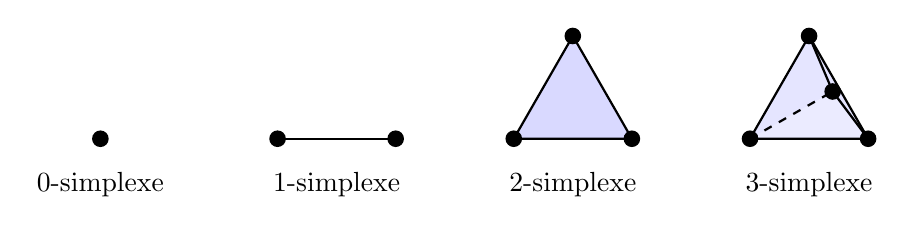
\begin{tikzpicture}[scale=1.5]
  % 0-simplex
  \fill (0,0) circle (2pt);
  \node[below] at (0,-0.2) {$0$-simplexe};
  % 1-simplex
  \draw[thick] (1.5,0) -- (2.5,0);
  \fill (1.5,0) circle (2pt);
  \fill (2.5,0) circle (2pt);
  \node[below] at (2,-0.2) {$1$-simplexe};
  % 2-simplex
  \fill[blue!15] (3.5,0) -- (4.5,0) -- (4,0.87) -- cycle;
  \draw[thick] (3.5,0) -- (4.5,0) -- (4,0.87) -- cycle;
  \fill (3.5,0) circle (2pt);
  \fill (4.5,0) circle (2pt);
  \fill (4,0.87) circle (2pt);
  \node[below] at (4,-0.2) {$2$-simplexe};
  % 3-simplex
  \fill[blue!10] (5.5,0) -- (6.5,0) -- (6,0.87) -- cycle;
  \fill[blue!8] (5.5,0) -- (6.5,0) -- (6.2,0.4) -- cycle;
  \draw[thick] (5.5,0) -- (6.5,0) -- (6,0.87) -- cycle;
  \draw[thick,dashed] (5.5,0) -- (6.2,0.4);
  \draw[thick] (6.5,0) -- (6.2,0.4);
  \draw[thick] (6,0.87) -- (6.2,0.4);
  \fill (5.5,0) circle (2pt);
  \fill (6.5,0) circle (2pt);
  \fill (6,0.87) circle (2pt);
  \fill (6.2,0.4) circle (2pt);
  \node[below] at (6,-0.2) {$3$-simplexe};
\end{tikzpicture}
\end{center}

\begin{definition}[Face]
Une \emph{face} d'un $p$-simplexe $\sigma = [v_0, \ldots, v_p]$ est
tout simplexe obtenu en supprimant un ou plusieurs sommets. La
\emph{$i$-\`eme face oppos\'ee} est~:
\[
  d_i \sigma = [v_0, \ldots, \hat{v}_i, \ldots, v_p]
\]
o\`u $\hat{v}_i$ indique l'omission du sommet $v_i$.
\end{definition}

% ============================================================
\section{Complexes simpliciaux abstraits}
% ============================================================

\begin{definition}[Complexe simplicial abstrait]
Un \emph{complexe simplicial abstrait} est une paire $K = (V, \Sigma)$
o\`u $V$ est un ensemble fini de sommets et $\Sigma \subseteq 2^V$ est
une collection de sous-ensembles non vides de $V$ telle que~:
\begin{enumerate}
  \item Pour tout $v \in V$, $\{v\} \in \Sigma$.
  \item Si $\sigma \in \Sigma$ et $\tau \subseteq \sigma$ avec
        $\tau \neq \emptyset$, alors $\tau \in \Sigma$.
\end{enumerate}
Les \'el\'ements de $\Sigma$ sont appel\'es \emph{simplexes} et la
condition~(2) est la \emph{propri\'et\'e de fermeture par faces}.
\end{definition}

\begin{definition}[Dimension]
La \emph{dimension} d'un simplexe $\sigma$ est $\dim \sigma = \abs{\sigma} - 1$.
La \emph{dimension} du complexe est $\dim K = \max_{\sigma \in \Sigma} \dim \sigma$.
\end{definition}

\begin{exemple}
Consid\'erons $V = \{a, b, c, d\}$ et~:
\[
  \Sigma = \big\{
    \{a\}, \{b\}, \{c\}, \{d\},
    \{a,b\}, \{b,c\}, \{a,c\}, \{c,d\},
    \{a,b,c\}
  \big\}.
\]
C'est un complexe simplicial de dimension~$2$. Il contient un
$2$-simplexe $\{a,b,c\}$ (triangle plein), quatre $1$-simplexes
(ar\^etes) et quatre $0$-simplexes (sommets).
\end{exemple}

% ============================================================
\section{Cha\^{\i}nes, bords et cycles}
% ============================================================

Fixons un corps $\mathbb{F}$ (typiquement $\mathbb{F}_2 = \Z / 2\Z$).

\begin{definition}[Groupe des cha\^{\i}nes]
Le \emph{groupe des $p$-cha\^{\i}nes} de $K$ \`a coefficients dans
$\mathbb{F}$ est l'espace vectoriel~:
\[
  C_p(K; \mathbb{F}) = \bigoplus_{\sigma \in \Sigma,\, \dim \sigma = p}
  \mathbb{F} \cdot \sigma.
\]
Un \'el\'ement de $C_p$ est une combinaison lin\'eaire formelle de
$p$-simplexes.
\end{definition}

\begin{definition}[Op\'erateur bord]
L'\emph{op\'erateur bord} $\partial_p : C_p(K) \to C_{p-1}(K)$ est
d\'efini sur les g\'en\'erateurs par~:
\[
  \partial_p [v_0, \ldots, v_p]
  = \sum_{i=0}^{p} (-1)^i [v_0, \ldots, \hat{v}_i, \ldots, v_p].
\]
\end{definition}

\begin{formules}[title=\textbf{Propri\'et\'e fondamentale du bord}]
\[
  \partial_{p-1} \circ \partial_p = 0 \quad \forall\, p.
\]
En d'autres termes, \emph{le bord d'un bord est nul}.
\end{formules}

\begin{proposition}
Pour tout $p \geq 0$, on a $\partial_{p-1} \circ \partial_p = 0$.
\end{proposition}

\begin{proof}
Soit $\sigma = [v_0, \ldots, v_p]$. Alors~:
\begin{align*}
\partial_{p-1}(\partial_p \sigma)
&= \partial_{p-1}\left(\sum_{i=0}^p (-1)^i
   [v_0,\ldots,\hat{v}_i,\ldots,v_p]\right) \\
&= \sum_{i=0}^p (-1)^i \sum_{\substack{j=0 \\ j \neq i}}^p (-1)^{j'}
   [v_0,\ldots,\hat{v}_j,\ldots,\hat{v}_i,\ldots,v_p]
\end{align*}
o\`u $j' = j$ si $j < i$ et $j' = j-1$ si $j > i$. Chaque terme
appara\^{\i}t exactement deux fois avec des signes oppos\'es, donc la
somme est nulle.
\end{proof}

\begin{definition}[Cycles et bords]
\begin{itemize}
  \item Le groupe des \emph{$p$-cycles} est $Z_p(K) = \ker \partial_p$.
  \item Le groupe des \emph{$p$-bords} est $B_p(K) = \mathrm{im}\, \partial_{p+1}$.
  \item Comme $\partial_{p} \circ \partial_{p+1} = 0$, on a
        $B_p(K) \subseteq Z_p(K)$.
\end{itemize}
\end{definition}

% ============================================================
\section{Homologie simpliciale}
% ============================================================

\begin{definition}[Groupe d'homologie]
Le \emph{$p$-i\`eme groupe d'homologie} de $K$ \`a coefficients dans
$\mathbb{F}$ est le quotient~:
\[
  H_p(K; \mathbb{F}) = Z_p(K) / B_p(K)
  = \ker \partial_p \,/\, \mathrm{im}\, \partial_{p+1}.
\]
Le \emph{$p$-i\`eme nombre de Betti} est
$\beta_p = \dim_\mathbb{F} H_p(K; \mathbb{F})$.
\end{definition}

\begin{formules}[title=\textbf{Formule des nombres de Betti}]
\[
  \beta_p = \dim \ker \partial_p - \dim \mathrm{im}\, \partial_{p+1}
  = \mathrm{rang}(Z_p) - \mathrm{rang}(B_p).
\]
\end{formules}

\begin{theoreme}[Caract\'eristique d'Euler--Poincar\'e]
Si $K$ est un complexe simplicial de dimension $d$, sa
\emph{caract\'eristique d'Euler} v\'erifie~:
\[
  \chi(K) = \sum_{p=0}^{d} (-1)^p \abs{\Sigma_p}
  = \sum_{p=0}^{d} (-1)^p \beta_p
\]
o\`u $\Sigma_p$ d\'esigne l'ensemble des $p$-simplexes de $K$.
\end{theoreme}

% ============================================================
\section{Calcul matriciel de l'homologie}
% ============================================================

En pratique, le calcul de l'homologie se ram\`ene \`a de l'alg\`ebre
lin\'eaire. Fixons un ordre sur les simplexes de chaque dimension.
L'op\'erateur $\partial_p$ est alors repr\'esent\'e par une matrice
$D_p$ \`a coefficients dans $\mathbb{F}$.

\begin{algorithme}[title=\textbf{Calcul des nombres de Betti}]
\begin{enumerate}
  \item Construire les matrices de bord $D_p$ pour $p = 1, \ldots, d$.
  \item Calculer $r_p = \mathrm{rang}(D_p)$ (par r\'eduction de Smith
        ou \'elimination de Gauss sur $\mathbb{F}$).
  \item Les nombres de Betti sont~:
        $\beta_p = \abs{\Sigma_p} - r_p - r_{p+1}$.
\end{enumerate}
\end{algorithme}

\begin{codeblock}[title=\textbf{Calcul de l'homologie avec des matrices}]
\begin{minted}{python}
import numpy as np

def boundary_matrix(simplices_p, simplices_pm1):
    """Matrice de bord sur F_2."""
    n_rows = len(simplices_pm1)
    n_cols = len(simplices_p)
    D = np.zeros((n_rows, n_cols), dtype=int)
    idx_map = {tuple(s): i for i, s in enumerate(simplices_pm1)}
    for j, sigma in enumerate(simplices_p):
        for k in range(len(sigma)):
            face = tuple(sigma[:k] + sigma[k+1:])
            if face in idx_map:
                D[idx_map[face], j] = 1  # mod 2
    return D % 2

def betti_numbers_f2(K, dim):
    """Calcule beta_0, ..., beta_dim sur F_2."""
    simplices_by_dim = {}
    for s in K:
        d = len(s) - 1
        simplices_by_dim.setdefault(d, []).append(sorted(s))
    bettis = []
    for p in range(dim + 1):
        sp = simplices_by_dim.get(p, [])
        if p > 0:
            D_p = boundary_matrix(sp, simplices_by_dim.get(p-1, []))
            rk_p = np.linalg.matrix_rank(D_p) if D_p.size else 0
        else:
            rk_p = 0
        sp1 = simplices_by_dim.get(p+1, [])
        if sp1:
            D_p1 = boundary_matrix(sp1, sp)
            rk_p1 = np.linalg.matrix_rank(D_p1) if D_p1.size else 0
        else:
            rk_p1 = 0
        bettis.append(len(sp) - rk_p - rk_p1)
    return bettis
\end{minted}
\end{codeblock}

% ============================================================
\section{Exemples de calcul}
% ============================================================

\begin{exemple}[Triangle creux]
Soit $K$ le complexe form\'e de trois sommets $\{a, b, c\}$ et trois
ar\^etes $\{a,b\}, \{b,c\}, \{a,c\}$, \emph{sans} le $2$-simplexe
$\{a,b,c\}$.
\begin{itemize}
  \item $D_1 = \begin{pmatrix} 1 & 0 & 1 \\ 1 & 1 & 0 \\ 0 & 1 & 1 \end{pmatrix}$
        (sur $\mathbb{F}_2$), de rang~$2$.
  \item $\beta_0 = 3 - 2 = 1$ (une composante connexe).
  \item $\beta_1 = 3 - 2 - 0 = 1$ (un trou --- le triangle est creux).
\end{itemize}
\end{exemple}

\begin{exemple}[Triangle plein]
Ajoutons le $2$-simplexe $\{a,b,c\}$ au complexe pr\'ec\'edent.
$D_2$ est le vecteur colonne $(1, 1, 1)^T$ sur $\mathbb{F}_2$,
de rang~$1$.
\begin{itemize}
  \item $\beta_0 = 3 - 2 = 1$.
  \item $\beta_1 = 3 - 2 - 1 = 0$ (le trou est rempli).
  \item $\beta_2 = 1 - 1 = 0$.
\end{itemize}
\end{exemple}

% ============================================================
\section{Homologie relative et suites exactes}
% ============================================================

\begin{definition}[Homologie relative]
Soit $L \subseteq K$ un sous-complexe. L'\emph{homologie relative} est~:
\[
  H_p(K, L; \mathbb{F}) = \ker(\bar{\partial}_p) / \mathrm{im}(\bar{\partial}_{p+1})
\]
o\`u $\bar{\partial}_p$ est induit par $\partial_p$ sur le quotient
$C_p(K)/C_p(L)$.
\end{definition}

\begin{theoreme}[Suite exacte longue du couple]
Il existe une suite exacte longue~:
\[
  \cdots \to H_p(L) \xrightarrow{i_*} H_p(K)
  \xrightarrow{j_*} H_p(K, L)
  \xrightarrow{\partial_*} H_{p-1}(L) \to \cdots
\]
\end{theoreme}

% ============================================================
\section{Homologie avec GUDHI}
% ============================================================

\begin{codeblock}[title=\textbf{Calcul d'homologie avec GUDHI}]
\begin{minted}{python}
import gudhi

# Construire un complexe simplicial
st = gudhi.SimplexTree()
st.insert([0, 1])
st.insert([1, 2])
st.insert([0, 2])
# Triangle creux: pas de 2-simplexe [0,1,2]

# Nombres de Betti
betti = st.betti_numbers()
print(f"Nombres de Betti: {betti}")
# Sortie: Nombres de Betti: {0: 1, 1: 1}

# Maintenant, remplir le triangle
st.insert([0, 1, 2])
betti = st.betti_numbers()
print(f"Nombres de Betti: {betti}")
# Sortie: Nombres de Betti: {0: 1}
\end{minted}
\end{codeblock}

% ============================================================
\section{Homologie r\'eduite et caract\'eristique d'Euler}
% ============================================================

\begin{definition}[Homologie r\'eduite]
L'\emph{homologie r\'eduite} $\tilde{H}_p(K)$ est d\'efinie en
augmentant le complexe de cha\^{\i}nes par l'application
$\varepsilon : C_0(K) \to \mathbb{F}$, $\varepsilon(\sum \lambda_i v_i)
= \sum \lambda_i$. On a~:
\[
  \tilde{H}_p(K) = \begin{cases}
    H_p(K) & \text{si } p > 0, \\
    \ker(\varepsilon) / B_0(K) & \text{si } p = 0.
  \end{cases}
\]
En particulier, $\tilde{\beta}_0 = \beta_0 - 1$ pour un complexe
non vide.
\end{definition}

% ============================================================
\section{Applications simpliciales et fonctorialit\'e}
% ============================================================

\begin{definition}[Application simpliciale]
Soient $K$ et $L$ deux complexes simpliciaux. Une \emph{application
simpliciale} $f : K \to L$ est une application $f : V_K \to V_L$ sur
les sommets telle que pour tout simplexe $\sigma = \{v_0, \ldots, v_p\}
\in K$, on ait $f(\sigma) = \{f(v_0), \ldots, f(v_p)\} \in L$.
\end{definition}

\begin{proposition}
Toute application simpliciale $f : K \to L$ induit une application
lin\'eaire $f_* : H_p(K) \to H_p(L)$ pour tout $p$. Cette assignation
est fonctorielle~: $(g \circ f)_* = g_* \circ f_*$ et
$(\mathrm{id}_K)_* = \mathrm{id}_{H_p(K)}$.
\end{proposition}

% ============================================================
\section{Exercices}
% ============================================================

\begin{exercice}
Calculer \`a la main les nombres de Betti du complexe simplicial form\'e
par les faces d'un t\'etra\`edre (sans l'int\'erieur). V\'erifier la
formule de la caract\'eristique d'Euler.
\end{exercice}

\begin{exercice}
Montrer que pour un graphe connexe $G$ avec $n$ sommets et $m$ ar\^etes,
$\beta_0 = 1$ et $\beta_1 = m - n + 1$.
\end{exercice}

\begin{exercice}
Impl\'ementer en Python la construction de la matrice de bord
$D_1$ pour un graphe donn\'e par sa liste d'ar\^etes. V\'erifier que
$D_0 \cdot D_1 = 0$ (sur $\mathbb{F}_2$) sur un exemple.
\end{exercice}

\begin{exercice}
Calculer l'homologie de la bouteille de Klein triangul\'ee (9 sommets,
27 ar\^etes, 18 triangles). Comparer les r\'esultats sur $\mathbb{F}_2$
et sur $\Q$.
\end{exercice}

\begin{exercice}
Montrer que si $K$ est un c\^one (i.e., il existe un sommet $v$ tel que
$\sigma \cup \{v\} \in K$ pour tout $\sigma \in K$), alors
$\tilde{H}_p(K) = 0$ pour tout $p$.
\end{exercice}
